%%%%%%%%%%%%%%%%%%%%%%%%%%%%%%%%%%%%%%%%%%%%%%%%%%%%%%%%%%%%%%%%%%%%%
%
% CS 172 Writeup Template
%
% This is a LaTeX document. LaTeX is a markup language for producing
% documents. Your task is to fill out this
% document, then to compile this into a PDF document.
% You will then upload this PDF to `Gradescope' - the grading system
% that we use.
%
%
% TO COMPILE:
% > pdflatex thisfile.tex
%
% For references to appear correctly instead of as '??', you must run
% pdflatex twice.
%
% If you do not have LaTeX and need a LaTeX distribution:
% - Departmental machines have one installed.
% - Personal laptops (all common OS): www.latex-project.org/get/
%
% If you need help with LaTeX, please come to office hours.
% Or, there is plenty of help online:
% https://en.wikibooks.org/wiki/LaTeX
%
%
%%%%%%%%%%%%%%%%%%%%%%%%%%%%%%%%%%%%%%%%%%%%%%%%%%%%%%%%%%%%%%%%%%%%%
%
% How to include two graphics on the same line:
%
% \includegraphics[\width=0.49\linewidth]{yourgraphic1.png}
% \includegraphics[\width=0.49\linewidth]{yourgraphic2.png}
%
% How to include equations:
%
% \begin{equation}
% y = mx+c
% \end{equation}
%
%%%%%%%%%%%%%%%%%%%%%%%%%%%%%%%%%%%%%%%%%%%%%%%%%%%%%%%%%%%%%%%%%%%%%%%%%%%%%%%%%%%%%%%%%%%%%%%%

\documentclass[11pt]{article}

\usepackage[english]{babel}
\usepackage[utf8]{inputenc}
\usepackage[colorlinks = true,
            linkcolor = blue,
            urlcolor  = blue]{hyperref}
\usepackage[a4paper,margin=1.5in]{geometry}
\usepackage{stackengine,graphicx}
\usepackage{fancyhdr}
\setlength{\headheight}{15pt}
\usepackage{microtype}
\usepackage{times}
\usepackage{booktabs}

% From https://ctan.org/pkg/matlab-prettifier
\usepackage[numbered,framed]{matlab-prettifier}

\frenchspacing
\setlength{\parindent}{0cm} % Default is 15pt.
\setlength{\parskip}{0.3cm plus1mm minus1mm}

\pagestyle{fancy}
\fancyhf{}
\lhead{Computer Vision: Project 1}
\rhead{CS172}
\rfoot{\thepage}

\title{\vspace{-1cm}Project 1 Report}
\author{Deng Chenguang \\ 85907286}
\date{\today}


\begin{document}
\maketitle
\vspace{-1.5cm}
\thispagestyle{fancy}

\section*{Introduction}
This report mainly cover how to implement a "Einstein-Marilyn" (or a "dog-cat") picture, by image filtering and hybrid images. In this task we abandon the matlab's \textit{imfilter} function but to rewrite our own \textit{my\_filter} function.


\section*{Procedure}
The most important task is to implement a filter that does convolution. \\But... What is a convolution? 
\begin{itemize}
	\item Read image and filter information first.
	\item Pad the image to a larger size for convolution.
	\item Rotate 180° and place the filter at the origin.
	\item Do convolution, the current pixel's value is the sum of all neighbours and filter's dot product, in each color channel.
	\item Move the filter row by row, column by column, s.t. its center covers every pixel.
	\item Ok, got the new image!
\end{itemize}
If you want a math explanation of what I have done, here it comes:
\begin{equation}
g=f*h
\end{equation} 
\begin{equation}
g(i,j)=\sum_{k,l}f(i-k,j-l)h(k,l)=\sum_{k,l}f(k,l)h(i-k,j-l)
\end{equation}
:)

\section*{Interesting Implementation Detail}
\begin{itemize}
	\item[(a)] \textbf{What is the upper bond and the lower bond?}\\
	Boundary handling can be tricky as the filter can't be centered on pixels. So we implement a new function called \textit{fil} to help us read the surrounding pixel's value of a pixel with the size of filter and do dot product.
	
	\begin{lstlisting}[style=Matlab-editor]
	
function new_pixel_val = fil(data, input_image, filter)
filter_height = size(filter,1);
filter_width = size(filter,2);

colors = data(3);

row_low = data(1) - floor(filter_height/2);
col_low = data(2) - floor(filter_width/2);
row_upp = data(1) + floor(filter_height/2);
col_upp = data(2) + floor(filter_width/2);

sub_mat = input_image(row_low:row_upp, col_low:col_upp, colors);

new_pixel_val = sum(sum(sub_mat.*filter));
end
	\end{lstlisting}
	In this we do not touch the original picture, but to copy the values we need to \textbf{sub\_mat}, and do dot product.
	\item[(b)] \textbf{What's the difference between convolution and correlation filter?}
	\\
	First, their names are different.\\
	Second, their equation are different.\\
	\begin{equation}
	g=f\otimes h
	\end{equation}
	i.e.
	\begin{equation}
g(i,j)=\sum_{k,l}f(i+k,j+l)h(k,l)
	\end{equation}
	Third, their final result may be different.
\end{itemize}

\section*{Result}

\begin{figure}[h]
    \centering
    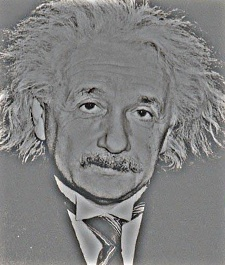
\includegraphics[width=5cm]{high_frequencies.jpg}
    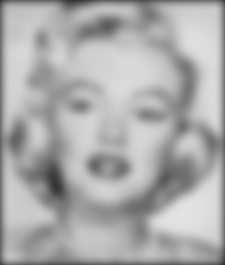
\includegraphics[width=5cm]{low_frequencies.jpg}
    \caption{\emph{Left:} Detail of Einstein. \emph{Right:} Smooth content of Marilyn.}
    \label{fig:result1}
\end{figure}

\begin{figure}
	\centering
	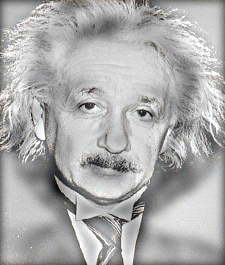
\includegraphics[width=0.5\linewidth]{hybrid_image}
	\caption{Combination.}
	\label{fig:hybridimage}
\end{figure}

\begin{figure}
	\centering
	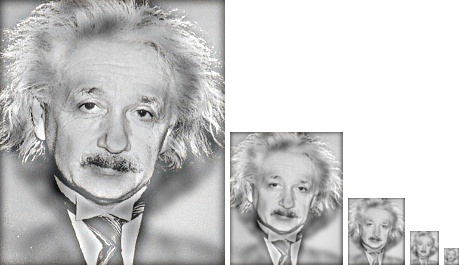
\includegraphics[width=0.9\linewidth]{hybrid_image_scales}
	\caption{Left is Einstein, right is Marilyn.}
	\label{fig:hybridimagescales}
\end{figure}




\end{document}
